\subsection{Importing bitmap graph}
The simplest method to import get your Octave/Matlab graphs onto a document is to export them to a bitmap picture, and import like we did before.

Our code looks something like the following\footnotemark, and the full example is in \verb|Examples/Importing-graphs|.
\lstinputlisting[language=Matlab, caption={\texttt{Importing-graphs/bitmap/example.m}}]{Examples/Importing-graphs/bitmap/bitmap-code.m}
\footnotetext{You may notice the figure is exported to \texttt{.eps}, not \texttt{.png}, \texttt{.tiff} or something otherwise more common. For that you may want to look into \href{https://uk.mathworks.com/matlabcentral/fileexchange/23629-export_fig}{\texttt{export\_fig}}.}

Then, to include the graph, we simply use \verb|\includegraphics|.
\begin{lstlisting}
\begin{figure}[h]
    \centering
    \includegraphics[width=\textwidth]{figures/example.eps}
\end{figure}
\end{lstlisting}
Below you can see the output compared to something natively drawn with pgfplots.
It is a deliberately simple graph that can be easily replicated natively, but it highlights that font sizes and other small issues can become problematic for legibility.

\begin{figure}[h]
\centering
\begin{minipage}{0.50\textwidth}
    \includegraphics[width=\textwidth]{Examples/Importing-graphs/bitmap/figures/example.eps}
    \caption{Matlab}
\end{minipage}
\hfill
\begin{minipage}{0.48\textwidth}
    \begin{tikzpicture}[]
        \begin{axis}[xlabel= \( x \), ylabel = \( f(x) \) ]
            \addplot[domain=0:2*pi, samples=100, blue] {sin(deg(x))};
            \legend{ \( f(x) = \sin(x)  \) }
        \end{axis}
    \end{tikzpicture}
    \caption{Natively rendered}
\end{minipage}
\end{figure}

So what can we do instead? We can generate the graphs in Octave/Matlab and export the data for \texttt{tikz} and \texttt{pgfplots} to natively render it.
We have two options to do so: \texttt{matlab2tikz} and exporting to a \texttt{.svg} file.

\paragraph{Challenge:}
Replicate the sinusoidal graph with \texttt{pgfplots}, and you might see a straight line, indicating that it uses degrees, not radians.
Try to search for the solution!
Hopefully you will run into \href{https://tex.stackexchange.com/questions/16232/how-to-plot-fx-sinx-kx-cosx-and-ux-x%C2%B2-with-tikz}{this} link.

\subsection{Matlab2tikz}
This is an outstanding script written by Nico Schlömer which can be downloaded from Mathworks' \href{https://uk.mathworks.com/matlabcentral/fileexchange/22022-matlab2tikz-matlab2tikz}{file exchange}, or directly from the \href{https://github.com/matlab2tikz/matlab2tikz}{github}. Please refer to the installation on the github page, if you are unfamiliar with installing external matlab functions.
In short, use Set Path to include the downloaded \verb|src/| to your path.

Usage is very similar to exporting a bitmap image, the only difference is that we get a \texttt{.tex} to import, which can be further edited if you really want to:
\lstinputlisting[language=Matlab, caption={\texttt{Importing-graphs/matlab2tikz/mat2tikz.m}}]{Examples/Importing-graphs/matlab2tikz/mat2tikz.m}

Importing requires a few packages and settings, as can be seen below.
The information is extracted from \texttt{matlab2tikz}'s github, and reading their \href{https://github.com/matlab2tikz/matlab2tikz/wiki/FAQ}{FAQ} may be very helpful 

The code is not separated into preamble and content, but it should be clear what goes where.
Importantly, the whole example can be found in \texttt{Examples/Importing-graphs}.
\lstinputlisting[language=tex, caption={\texttt{Importing-graphs/matlab2tikz/totikz.tex}}]{Examples/Importing-graphs/matlab2tikz/totikz.tex}
Resulting in:
\begin{figure}[h]\centering
\begin{minipage}{0.49\textwidth}
    \newlength\fheight{} \newlength\fwidth{}
    \setlength\fheight{5.5cm}
    \setlength\fwidth{7cm}    
% This file was created by matlab2tikz.
%
%The latest updates can be retrieved from
%  http://www.mathworks.com/matlabcentral/fileexchange/22022-matlab2tikz-matlab2tikz
%where you can also make suggestions and rate matlab2tikz.
%
\definecolor{mycolor1}{rgb}{0.00000,0.44700,0.74100}%
%
\begin{tikzpicture}

\begin{axis}[%
width=0.951\fwidth,
height=\fheight,
at={(0\fwidth,0\fheight)},
scale only axis,
xmin=0,
xmax=7,
xlabel style={font=\color{white!15!black}},
xlabel={x},
ymin=-1,
ymax=1,
ylabel style={font=\color{white!15!black}},
ylabel={f(x)},
axis background/.style={fill=white},
legend style={legend cell align=left, align=left, draw=white!15!black}
]
\addplot [color=mycolor1]
  table[row sep=crcr]{%
0	0\\
0.0634665182543393	0.0634239196565645\\
0.126933036508679	0.126592453573749\\
0.190399554763018	0.18925124436041\\
0.253866073017357	0.251147987181079\\
0.317332591271696	0.312033445698487\\
0.380799109526036	0.371662455660328\\
0.444265627780375	0.429794912089172\\
0.507732146034714	0.486196736100469\\
0.571198664289053	0.540640817455598\\
0.634665182543393	0.59290792905464\\
0.698131700797732	0.642787609686539\\
0.761598219052071	0.690079011482112\\
0.82506473730641	0.734591708657533\\
0.88853125556075	0.776146464291757\\
0.951997773815089	0.814575952050336\\
1.01546429206943	0.849725429949514\\
1.07893081032377	0.881453363447582\\
1.14239732857811	0.909631995354518\\
1.20586384683245	0.934147860265107\\
1.26933036508679	0.954902241444074\\
1.33279688334112	0.971811568323542\\
1.39626340159546	0.984807753012208\\
1.4597299198498	0.993838464461254\\
1.52319643810414	0.998867339183008\\
1.58666295635848	0.999874127673875\\
1.65012947461282	0.996854775951942\\
1.71359599286716	0.989821441880933\\
1.7770625111215	0.978802446214779\\
1.84052902937584	0.963842158559942\\
1.90399554763018	0.945000818714669\\
1.96746206588452	0.922354294104581\\
2.03092858413886	0.895993774291336\\
2.0943951023932	0.866025403784439\\
2.15786162064753	0.832569854634771\\
2.22132813890187	0.795761840530832\\
2.28479465715621	0.755749574354258\\
2.34826117541055	0.712694171378863\\
2.41172769366489	0.666769000516292\\
2.47519421191923	0.618158986220605\\
2.53866073017357	0.567059863862771\\
2.60212724842791	0.513677391573407\\
2.66559376668225	0.458226521727411\\
2.72906028493659	0.400930535406614\\
2.79252680319093	0.342020143325669\\
2.85599332144527	0.28173255684143\\
2.91945983969961	0.220310532786541\\
2.98292635795395	0.15800139597335\\
3.04639287620828	0.0950560433041829\\
3.10985939446262	0.0317279334980681\\
3.17332591271696	-0.0317279334980679\\
3.2367924309713	-0.0950560433041826\\
3.30025894922564	-0.15800139597335\\
3.36372546747998	-0.220310532786541\\
3.42719198573432	-0.281732556841429\\
3.49065850398866	-0.342020143325669\\
3.554125022243	-0.400930535406613\\
3.61759154049734	-0.45822652172741\\
3.68105805875168	-0.513677391573406\\
3.74452457700602	-0.567059863862771\\
3.80799109526036	-0.618158986220605\\
3.87145761351469	-0.666769000516292\\
3.93492413176903	-0.712694171378863\\
3.99839065002337	-0.755749574354258\\
4.06185716827771	-0.795761840530832\\
4.12532368653205	-0.832569854634771\\
4.18879020478639	-0.866025403784438\\
4.25225672304073	-0.895993774291336\\
4.31572324129507	-0.922354294104581\\
4.37918975954941	-0.945000818714668\\
4.44265627780375	-0.963842158559942\\
4.50612279605809	-0.978802446214779\\
4.56958931431243	-0.989821441880933\\
4.63305583256677	-0.996854775951942\\
4.69652235082111	-0.999874127673875\\
4.75998886907544	-0.998867339183008\\
4.82345538732978	-0.993838464461254\\
4.88692190558412	-0.984807753012208\\
4.95038842383846	-0.971811568323542\\
5.0138549420928	-0.954902241444074\\
5.07732146034714	-0.934147860265107\\
5.14078797860148	-0.909631995354519\\
5.20425449685582	-0.881453363447582\\
5.26772101511016	-0.849725429949514\\
5.3311875333645	-0.814575952050336\\
5.39465405161884	-0.776146464291757\\
5.45812056987318	-0.734591708657534\\
5.52158708812751	-0.690079011482113\\
5.58505360638185	-0.64278760968654\\
5.64852012463619	-0.59290792905464\\
5.71198664289053	-0.540640817455597\\
5.77545316114487	-0.486196736100469\\
5.83891967939921	-0.429794912089172\\
5.90238619765355	-0.371662455660328\\
5.96585271590789	-0.312033445698487\\
6.02931923416223	-0.251147987181079\\
6.09278575241657	-0.189251244360411\\
6.15625227067091	-0.12659245357375\\
6.21971878892525	-0.0634239196565654\\
6.28318530717959	-2.44929359829471e-16\\
};
\addlegendentry{f(x)=sin(x)}

\end{axis}
\end{tikzpicture}%
\caption{Matlab generated and rendered natively}
\end{minipage}
\hfill
\begin{minipage}{0.49\textwidth}
    \begin{tikzpicture}[]
        \begin{axis}[xlabel= \( x \), ylabel = \( f(x) \),
            ymin=-1, xmin=0, ymax=1,]
            \addplot[domain=0:2*pi, samples=100, blue] {sin(deg(x))};
            \legend{ \( f(x) = \sin(x)  \) }
        \end{axis}
    \end{tikzpicture}
    \caption{Generated with pgfplots}
\end{minipage}
\end{figure}

Do you know why the fonts look still different? In the graph generated by matlab, we did not tell it to render using math mode --- f(x) vs \( f(x) \).

\subsection{Importing vector graph}